\clearpage
\section{Quantum Phenomena and Entanglement}
  \label{sec:quantum-phenomena-and-entanglement}

  \paragraph{Scope and strategy.}
    This section explains how quantum phenomenology can arise as an effective statistical description
    of the projection process itself.
    The key structural ingredient is the \emph{non-injective} character of the projection $\Pi$:
    distinct underlying $\chi$-configurations can correspond to the same effective observables,
    and a single underlying configuration may admit multiple effective images.
    We emphasize an \textbf{Ontological Monism} viewpoint: there is a single ontological source $\chi$,
    while apparent multiplicity and spatial separation are properties of the projected description.
    Within this setting, ``nonlocality'' does not require any signal transmission, because the correlated outcomes
    do not originate from independent ontological subsystems.

  \subsection{Non-Injective Projection as the Origin of Quantum Correlations}
  \label{subsec:non-injective-projection}

  The emergence of quantum correlations and entanglement in the Cosmochrony
  framework is rooted in a single structural property of the projection from
  the fundamental $\chi$ substrate to effective physical descriptions:
  this projection is \emph{non-injective}.

  A single admissible configuration of $\chi$ may correspond to multiple
  distinct effective degrees of freedom.
  What appear, at the effective level, as separate particles or subsystems
  are therefore multiple projective manifestations of a single underlying
  ontological configuration.

  This non-injectivity implies that such degrees of freedom cannot be assigned
  independent states.
  Any admissible effective description must be globally consistent with the
  underlying $\chi$ configuration, leading to persistent correlations that
  do not rely on signal exchange, causal influence, or spacetime proximity.

\subsubsection*{Ontological Monism and the Shared Projection Hypothesis}
  \label{subsec:ontological-monism-shared-projection}

  In Cosmochrony, the apparent multiplicity of effective particles does not imply a multiplicity of
  ontological entities.
  The framework adopts \textbf{Ontological Monism}: there is a single ontological source, the substrate $\chi$.
  What appears as ``two systems'' in spacetime may correspond to a single underlying relational configuration.

  \paragraph{Shared projection hypothesis.}
    Because the projection $\Pi$ is non-injective and may admit multiple effective images,
    a single connected excitation in $\chi$ can be represented as several spatially separated effective
    excitations in the emergent description.
    The observed separation is therefore a property of the projected metric representation,
    not a fundamental separation of the underlying entity.

  \paragraph{Shared Fiber Phase and a Geometric Reading of Spin Correlations}
    \label{subsec:shared-fiber-phase-spin}

    In the Cosmochrony interpretation, spin correlations can be read as correlations of a \emph{shared}
    internal degree of freedom of the projection fiber, rather than as correlations between independent
    spacetime-local properties.
    When an entangled pair admits a description as multiple effective images of a single underlying
    $\chi$-configuration (Section~\ref{subsec:ontological-monism-shared-projection}), a measurement at one location
    selects a locally stable reprojection of that shared fiber degree of freedom.
    The correlated statistics at the distant location then reflect the restricted set of reprojections
    still compatible with the same underlying configuration, without invoking any signal exchange.

    This viewpoint is compatible with the emergence of half-integer spin from nontrivial fiber topology
    (e.g.\ Hopf-type structures), while keeping the explanation at the structural level: the relevant
    degrees of freedom are global properties of the shared configuration, not attributes of the two
    effective particles taken separately.

  \paragraph{Consequence for nonlocal correlations.}
    Correlations between measurements performed at spacelike separated locations do not require any
    superluminal influence.
    They follow from the fact that the correlated outcomes are local reprojections of the \emph{same}
    underlying configuration.
    In this sense, the ``Bell tension'' is not resolved by a faster-than-light mechanism, but by denying
    the premise that two independent ontological subsystems existed in the first place.

  \input{08-quantum-correlations-and-entanglement/02-nonlocality-and-holistic-nature}
  \subsection{Nonlocal Correlations Without Superluminality}
  \label{subsec:nonlocal-correlations-without-superluminality}

  Within the Cosmochrony framework, nonlocal quantum correlations do not arise from
  superluminal propagation of information.
  All admissible projected descriptions respect local causal constraints, and no
  measurement outcome influences another through dynamical signal exchange.
  This absence of information transfer is not enforced by a relativistic prohibition alone,
  but reflects a deeper ontological fact:
  there is no transmission of information because, at the level of the $\chi$ substrate,
  there is no fundamental separation to bridge.
  What appear as distinct outcomes correspond to local reprojections of a single underlying relational configuration.

  Correlated outcomes instead arise because spacelike separated measurements correspond
  to different local reprojections of a single non-factorizable admissible projected description.
  Such descriptions cannot be decomposed into independent subsystems without loss of global consistency.
  This failure of factorization is not accidental, but reflects the absence of an
  injective mapping between effective subsystems and underlying $\chi$ configurations.
  As a result, the factorization assumptions underlying Bell-type inequalities are
  violated, while dynamical locality and relativistic causality remain intact.
  This point is grounded in the relational formulation, where factorization is not
  fundamental but only an approximate emergent feature of certain projectable regimes
  (see Appendix~E, especially Appendix~\ref{subsec:non-factorization-and-entanglement}.

  In this perspective, quantum correlations reflect global descriptive consistency
  rather than hidden variables or pre-existing local properties.
  Measurement outcomes do not reveal predetermined values, but correspond to compatible
  local realizations selected from a shared non-factorizable descriptive structure.
  Equivalently, admissible projected descriptions determine a constrained \emph{space}
  of mutually compatible local realizations, rather than a set of pre-assigned outcomes.

  Cosmochrony therefore accounts for experimentally observed violations of Bell
  inequalities without invoking nonlocal forces, retrocausality, or hidden signal channels.
  Nonlocality appears as a structural feature of admissible projected descriptions,
  fully compatible with relativistic causal constraints.
  A compact way to state this is that the correlations are \emph{ontological}, fixed by the non-injective global
  relational structure, rather than \emph{dynamical}, mediated by any superluminal interaction.

  \subsection{Relation to Bell Inequalities}
  \label{subsec:relation-to-bell-inequalities}

  Bell's theorem~\cite{Bell1964} establishes that no physical theory reproducing the full
  set of quantum mechanical predictions can simultaneously satisfy locality,
  realism understood as outcome determinism conditioned on hidden variables, and statistical independence.
  The empirical violations of Bell inequalities therefore rule out any ontological
  completion of quantum mechanics based on factorizable hidden-variable models.

  The Cosmochrony framework fully accepts Bell's theorem as a fundamental constraint.
  It does not seek to evade or weaken Bell inequalities, nor to restore locality or realism in their classical sense.
  Instead, it identifies the precise ontological assumption that fails within
  Bell-type derivations when applied to admissible projected descriptions.

  \paragraph{Failure of ontological factorisability.}
    Standard Bell-type arguments assume that joint outcome probabilities admit a factorization of the form
    \begin{equation}
      P(a,b|x,y,\lambda) = P(a|x,\lambda)\,P(b|y,\lambda),
    \end{equation}
    where $\lambda$ denotes a complete specification of the underlying ontic state.
    In Cosmochrony, such a decomposition is not available, not because of nonlocal dynamical influences, but because
    admissible projected descriptions are subject to global consistency constraints imposed by the projection
    $\Pi$ (Section~\ref{sec:relational_projection}).

    More precisely, the projection $\Pi$ is generically non-injective: multiple distinct configurations of the
    relational substrate $\chi$ may correspond to the same effective description.
    As a result, admissible projected states are not associated with independent ontic pre-images for their subsystems.
    Entangled systems therefore correspond to equivalence classes of non-separable configurations in $\chi$,
    for which no decomposition into independently specifiable local states exists.
    In this sense, the factorization hypothesis required by Bell-type inequalities is not merely violated,
    but is \emph{ill-defined} within the space of admissible projected descriptions.

  \paragraph{Projection-induced correlations and informational compression.}
    The failure of factorization can be understood as a structural consequence of the
    compressive character of the projection $\Pi$.
    The projection maps a high-dimensional relational configuration space onto a reduced
    effective description by discarding unresolved internal degrees of freedom.
    The corresponding projection fiber $\Pi^{-1}(\chi_{\mathrm{eff}})$ may therefore
    contain a large equivalence class of underlying configurations.

    When this compression is neither negligible nor overwhelming, residual global
    constraints persist across projected subsystems, giving rise to non-factorizable correlations.
    Bell-type violations thus arise naturally in an intermediate regime where the
    effective description is sufficiently coarse-grained to permit subsystem
    separation, yet not so coarse as to erase all global relational structure.
    In contrast, in the limit of extreme coarse-graining, projected descriptions become
    effectively factorized, recovering classical statistical behavior.

    In this view, quantum entanglement corresponds to a critical regime of projection:
    neither a direct reflection of the underlying relational configuration, nor a fully
    classical description obtained by over-compression.

    This critical regime and its interpretation in terms of projective compression are developed independently of Bell
    inequalities in Section~\ref{subsec:entanglement-critical-compression}, where entanglement is shown to arise as a
    structural consequence of non-injective projection rather than as a dynamical or measurement-induced effect.

  \begin{figure}[t]
      \centering
      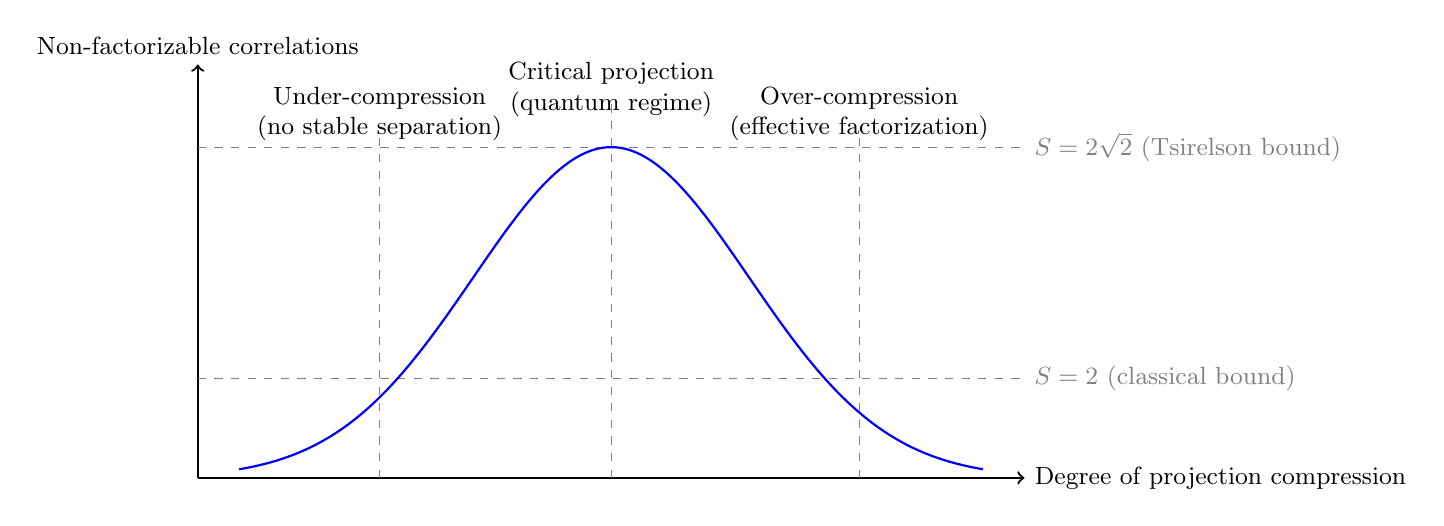
\begin{tikzpicture}[
        scale=1.05,
        axis/.style={->, thick},
        curve/.style={thick, smooth, blue},
        dashedline/.style={dashed, gray},
        label/.style={font=\small}
      ]

% Axes
        \draw[axis] (0,0) -- (10,0) node[right,label] {Degree of projection compression};
        \draw[axis] (0,0) -- (0,5) node[above,label] {Non-factorizable correlations};

% Bell bounds
        \draw[dashedline] (0,1.2) -- (10,1.2)
        node[right,label] {$S=2$ (classical bound)};
        \draw[dashedline] (0,4) -- (10,4)
        node[right,label] {$S=2\sqrt{2}$ (Tsirelson bound)};

% Bell-violation curve
        \draw[curve]
        plot[domain=0.5:9.5,samples=200]
        (\x,{4*exp(-0.18*(\x-5)^2)});

% Regime labels
        \node[label, align=center] at (2.2,4.4)
          {Under-compression\\(no stable separation)};
        \node[label, align=center] at (5,4.7)
          {Critical projection\\(quantum regime)};
        \node[label, align=center] at (8,4.4)
          {Over-compression\\(effective factorization)};

% Vertical guides
        \draw[dashedline] (2.2,0) -- (2.2,4.2);
        \draw[dashedline] (5,0) -- (5,4.6);
        \draw[dashedline] (8,0) -- (8,4.2);

      \end{tikzpicture}
      \caption{Schematic representation of Bell inequality violations as a function of the
      compression induced by the projection $\Pi$.
      Non-factorizable correlations emerge only in an intermediate regime, where the effective
      description is sufficiently coarse-grained to permit subsystem separation, yet retains
      enough global relational structure to prevent factorization.
      In the limit of over-compression, projected descriptions become effectively classical and
      Bell violations disappear.}
      \label{fig:bell-compression-regime}
    \end{figure}

  \paragraph{No hidden variables and no superluminal influence.}
    The absence of ontologically independent subsystems does not introduce hidden variables, local or nonlocal.
    The underlying degrees of freedom are neither accessible nor conditionable, and cannot
    be used to screen correlations or define outcome-determining parameters.
    Accordingly, the violation of Bell inequalities in Cosmochrony does not rely on
    superluminal signalling, retrocausality, or a breakdown of relativistic causal structure.

    Correlations are not mediated, transmitted, or dynamically generated between spatially separated subsystems.
    They reflect global admissibility constraints on projected descriptions, inherited
    from the holistic structure of the underlying configuration space.

  \paragraph{Ontological rather than dynamical nonlocality.}
    Quantum nonlocality in Cosmochrony is therefore ontological rather than dynamical.
    The failure of Bell-type factorizability arises from the structure of admissible
    projected descriptions themselves, not from any nonlocal interaction or exchange of information.
    Bell inequality violations are understood as a manifestation of non-separability
    under projection, rather than as evidence for superluminal causal influences.

    This interpretation preserves the full empirical content of quantum mechanics,
    respects relativistic causality at the operational level, and provides a structural
    explanation for the ubiquity and robustness of entanglement correlations within a
    non-injective relational framework.

  \paragraph{Structural scope of Bell violations.}
    The present analysis establishes the \emph{structural admissibility} of Bell inequality
    violations within Cosmochrony, by identifying the failure of ontological factorisability
    under non-injective projection.
    However, this result does not imply that non-factorizable correlations are uniformly
    realized across all projectable regimes.

    Bell inequalities constrain the logical form of admissible effective descriptions, but
    do not determine the conditions under which such correlations become dynamically or
    operationally accessible.
    The identification of specific regimes in which entanglement is activated, suppressed,
    or extinguished requires additional structural criteria beyond Bell’s theorem itself.

    These regime-dependent aspects of entanglement, including the role of projective
    compression and saturation effects, are addressed independently in
    Section~\ref{subsec:entanglement-critical-compression} and in the numerical investigations
    presented in Appendix~D.

  \subsection{Measurement, Decoherence, and Apparent Collapse}
  \label{subsec:measurement-and-decoherence}

  Within the Cosmochrony framework, quantum measurement does not involve a fundamental wavefunction collapse.
  At the fundamental level, no discontinuous update of the underlying relational substrate occurs.
  What is conventionally described as collapse arises entirely within the domain of effective projected descriptions.

  This is a direct consequence of the non-injective nature of the projection from the
  underlying $\chi$ substrate: multiple effective descriptions may correspond to a
  single relational configuration, with no uniquely defined inverse mapping.

  Measurement corresponds to the transition from a non-factorizable admissible
  projected description to a set of effectively factorized local projections.
  This transition is induced by interactions with an environment that progressively
  eliminate the accessibility of global relational coherence.
  As a result, alternative relational components cease to admit a joint effective
  description within a single spacetime representation.

  From this perspective, decoherence corresponds to an effective reduction of the
  multiplicity of admissible non-injective projections to a set of locally injective
  descriptions.

  Decoherence therefore does not represent a postulated measurement axiom, but a
  dynamical restriction on admissible projected descriptions~\cite{Zurek2003}.
  It suppresses interference between incompatible descriptive branches by rendering
  their relative phase information inaccessible within spacetime representations.
  The underlying relational structure remains globally well defined, even though it
  can no longer be represented coherently at the effective level.

  Importantly, decoherence does not destroy information.
  It limits the projectability of relational correlations into spacetime descriptions.
  In this sense, decoherence may be understood as a local and partial loss of
  projectability: certain relational distinctions persist structurally but cease to be
  jointly representable within an effective geometric description.

  More extreme regimes, such as those associated with strong gravitational confinement,
  represent a limiting case of this mechanism.
  In such regimes, not only coherence but spacetime representability itself breaks down.
  Relational information remains globally encoded, but undergoes a complete loss of
  spatiotemporal projectability, beyond the domain in which decoherence and effective
  Hilbert-space descriptions can be meaningfully defined.

  The apparent collapse observed in quantum measurement is therefore not a physical
  event, but the effective manifestation of a non-injective relational structure becoming
  only partially projectable into spacetime descriptions.

  \begin{tcolorbox}[
    colback=white,
    colframe=black!70,
    title={Do Quantum Particles Modify Their Past?},
    fonttitle=\bfseries
  ]
    It is sometimes claimed that quantum mechanics allows particles to
    \emph{modify their past}, particularly in delayed-choice or quantum eraser experiments.
    This statement is misleading.

    In quantum mechanics, physical descriptions are constrained globally by consistency conditions.
    Certain properties—such as path information or temporal ordering—do not possess
    well-defined values independently of the measurement context.
    A later measurement choice does not alter a previously existing physical fact,
    but rather restricts the set of admissible descriptions compatible with the entire experimental configuration.

    In the Cosmochrony framework, this behavior follows directly from the non-injective character of projection.
    A single underlying $\chi$ configuration may admit multiple effective
    descriptions, none of which defines a unique local past prior to measurement.
    The act of measurement does not modify the underlying relational structure;
    it reduces the multiplicity of admissible projections, rendering certain past properties effectively definable.

    Thus, quantum mechanics does not imply retrocausal influence or violations of relativistic causality.
    Instead, it reveals that some features commonly attributed to the past are not
    fundamental ontological facts, but emergent properties of admissible projected descriptions.
  \end{tcolorbox}

  \subsection{Temporal Ordering and Relativistic Consistency}
  \label{subsec:temporal-ordering-and-relativistic-consistency}

  Within the Cosmochrony framework, temporal ordering is not defined by a global notion of simultaneity.
  It arises only at the level of effective descriptions, as an ordering of admissible
  projected events induced by constrained relaxation ordering, rather than by any
  fundamental or absolute time parameter.

  This effective character of temporal ordering follows directly from the
  non-injective nature of the projection from the underlying $\chi$ substrate,
  for which no unique global temporal parametrization exists at the fundamental
  level.

  Different observers may therefore assign different temporal orderings to spacelike
  separated events within effective geometric descriptions.
  Such differences reflect the observer-dependence of spacetime slicing and have no
  impact on the underlying relational consistency of admissible projected descriptions.
  No preferred foliation, global clock, or absolute temporal structure is selected at the fundamental level.

  Entanglement correlations are thus fully compatible with relativistic causality.
  Because entangled correlations originate from a single underlying relational
  configuration, their consistency does not depend on any particular temporal
  ordering assigned within effective descriptions.
  They do not rely on any privileged reference frame or on a globally defined temporal ordering.
  Instead, they arise from non-factorizable admissible projected descriptions whose
  internal relational consistency is preserved under changes of effective spacetime coordinates and temporal slicings.

  In this sense, relativistic covariance is maintained because the physical content of
  the theory resides in relational consistency conditions rather than in observer-dependent spatiotemporal labels.
  Temporal ordering remains an effective, observer-relative notion, while admissible
  correlations and their consistency relations remain invariant across all equivalent projected descriptions.

  Relativistic covariance is therefore preserved not by enforcing a specific
  temporal structure, but by the invariance of the underlying non-injective
  relational configuration across all admissible projected descriptions.

  \begin{tcolorbox}[
    colback=white,
    colframe=black!70,
    title={Relation to Time-Symmetric and Two-State Vector Formulations},
    fonttitle=\bfseries
  ]
    Several time-symmetric formulations of quantum mechanics, such as the
    two-state vector formalism, account for delayed-choice and post-selection
    effects by introducing both forward- and backward-evolving quantum states.

    In the Cosmochrony framework, this apparent temporal symmetry is a consequence of
    \textbf{Ontological Monism}.
    All correlated outcomes originate from a single underlying $\chi$ configuration,
    rather than from dynamically interacting subsystems.
    What appears as spatial or temporal separation in effective descriptions does not
    correspond to a fundamental ontological separation.
    Consequently, no notion of information transmission—whether forward or backward
    in time—is required to account for quantum correlations.

    What time-symmetric approaches encode through boundary conditions imposed at
    both initial and final times is here recovered as a purely structural feature
    of admissible projected descriptions.
    The future does not influence the past; rather, effective temporal ordering
    does not exhaust the relational information contained in the underlying
    configuration.

    Time-symmetric formalisms thus appear as efficient descriptive tools within
    standard quantum mechanics, but they are not ontologically required once
    non-injective projection and irreversible relaxation are taken as fundamental.
  \end{tcolorbox}

  \input{08-quantum-correlations-and-entanglement/07-limits-of-entanglement}
  \input{08-quantum-correlations-and-entanglement/08-standard-model-integration}
  \subsection{Summary}
  \label{subsec:summary7}

  Within the Cosmochrony framework, particles are not fundamental entities.
  They emerge only at the level of effective descriptions, as stable and localized
  projected configurations that resist admissible relaxation ordering.
  Their physical properties are not postulated but arise as invariants of the
  structural and topological organization of admissible projected descriptions.

  Mass is identified with the degree of effective relaxation resistance encoded in a
  localized projected configuration.
  It quantifies how strongly such a configuration constrains admissible relaxation
  ordering relative to a homogeneous effective background.
  In regimes where a relativistic description applies, this interpretation naturally
  leads to the relation $E = mc^2$, understood as a kinematic identity rather than a
  fundamental postulate.

  Spin and statistical behavior originate from topological obstructions in the space
  of admissible projected configurations.
  Fermionic configurations exhibit a $4\pi$ periodicity in configuration space, such
  that a $2\pi$ rotation corresponds to a non-contractible loop and induces a sign
  change of the effective wavefunction.
  This topological structure provides a common origin for spin-$\tfrac{1}{2}$
  behavior, fermionic antisymmetry, and the Pauli exclusion principle
  without invoking additional quantum axioms.

  Within this perspective, different particle attributes correspond to distinct
  topological invariants of admissible projected descriptions.
  Spin is associated with non-trivial covering properties of configuration space,
  while electric charge may be interpreted, at an effective level, as an oriented
  topological defect or vortex-like structure within projected descriptions.
  These attributes remain conceptually distinct but arise from a common relational
  substrate once a geometric interpretation becomes meaningful.

  Taken together, these results provide a unified account of particle properties
  compatible with both relativistic and quantum phenomenology, without introducing
  particles or their attributes as fundamental ontological constituents.
  Particles appear instead as stable descriptive regimes of the underlying relational
  structure, whose properties reflect the topology of admissible projected
  configurations.

